\section{Modello di sviluppo}
	Come modello di sviluppo abbiamo deciso di utilizzare il \textbf{modello incrementale} (fig.\ref{fig::Model}) in quanto risulta essere il più adatto allo sviluppo della componente software a noi richiesta in relazione alle nostre capacità. 
	
	\subsection{Modello Incrementale}
		Il modello incrementale si basa sui seguenti passi:
		\begin{enumerate}
			\item pianificazione;
			\item analisi dei requisiti\pedice;
			\item progettazione;
			\item implementazione;
			\item validazione;
			\item valutazione.
		\end{enumerate}
		di cui i punti 2, 3, 4 e 5 possono essere eseguiti più volte, ma solo in maniera ciclica. Un approccio incrementale è consigliato quando la specifica dei requisiti risulta essere particolarmente difficoltosa e di difficile stesura, infatti questo modello favorisce lo sviluppo di prototipi che verranno utilizzati sia in fase di test che come anteprima per clienti.

		\begin{figure}[!htpb]
			\centering
		    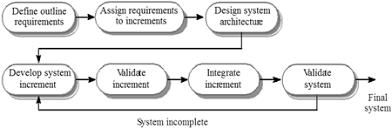
\includegraphics{IterativeModel.png}
			\caption{Modello incrementale}
			\label{fig::Model}
		\end{figure}

    \subsection{Incrementi}
        Gli incrementi saranno della durata massima di due settimane, e saranno così strutturati:
        \begin{itemize}
            \item Nel primo giorno verranno assegnati i compiti ad ogni membro del gruppo;
            \item Negli ultimi due giorni del periodo verificheremo i prodotti tramite i vari test di conformità alle aspettative;
            \item i restanti giorni saranno dedicati alla realizzazione dei componenti assegnati il primo giorno.
        \end{itemize}
        Con questa suddivisione temporale, il numero di incrementi previsti è limitato superiormente, come spiegheremo nella sezione \ref{Cap:Pianificazione}